% #############################################################################
% This is Chapter 2
% !TEX root = ../main.tex
% #############################################################################
% Change the Name of the Chapter i the following line
\fancychapter{Theoretical Background}
\cleardoublepage
% The following line allows to ref this chapter
\label{chapter:background}
Computer vision is a field of artificial intelligence that allows computers to understand, identify, and develop an intelligent understanding of digital images, just like human vision. It is used for many different tasks, most notably:

\begin{itemize}
    \item \textbf{Feature identification} in an image, such as edge detection;
    \item \textbf{Object detection} to classify all the different objects in an image along with their position;
    \item \textbf{Image segmentation}, i.e., assigning each pixel value in an image to a particular class;
    \item \textbf{Neural Style Transfer}, i.e., a new image is generated by learning the style from one image and applying it to another image.
\end{itemize}

In recent years, most tasks related to computer vision, such as those mentioned, have been solved using modern deep learning architectures, such as \ac{CNN} \cite{review:CV}. In this chapter, the main \ac{DL} algorithms developed for computer vision tasks, more specifically for image segmentation tasks, are explained in detail. 

\section{Convolutional Neural Networks}
\label{section:CNN&UNET}

%%%%%%%%%%%%%%%%%%%%%%%%%%%%%%%%%% CNN %%%%%%%%%%%%%%%%%%%%%%%%%%%%%%%%%%%%%

\subsection{CNN building blocks}

A Convolutional Neural Network is a class of \ac{NN} that specializes in processing data with a grid-like topology, such as images. Its built-in convolutional layer reduces the high dimensionality of images without losing their information. Therefore, \ac{CNNs} are best suitable for this use case.

A digital image is a binary representation of visual data. It contains a set of pixels arranged in a grid-like fashion and containing pixel values that indicate how bright and what color each pixel should be. 

A \ac{CNN} is typically composed of three types of layers: convolutional layers, pooling layers and fully connected layers. 

\subsubsection*{Convolutional Layer}

In a convolutional layer a filter or kernel "slides" over the input image and performs an element-wise dot product. As a result, it will be summing up the results into a single output pixel. The kernel will perform the same operation for every location it slides over, producing a two-dimensional representation of the image called a feature map. The size of the filters is usually smaller than the actual image, but the depth is equal to the number of channels \cite{2018guide}. Figure \ref{fig:convlayer} shows an example of the convolution process.

If we have an image with multiple channels (e.g. RGB images have 3 channels), we have one \ac{2D} kernel per input channel and we perform each convolution, of the \ac{2D} input channel with the \ac{2D} kernel, separately and then sum the contributions with the bias, resulting in the final output feature map \cite{2018guide}.

\begin{figure}[!htb]
  \centering
  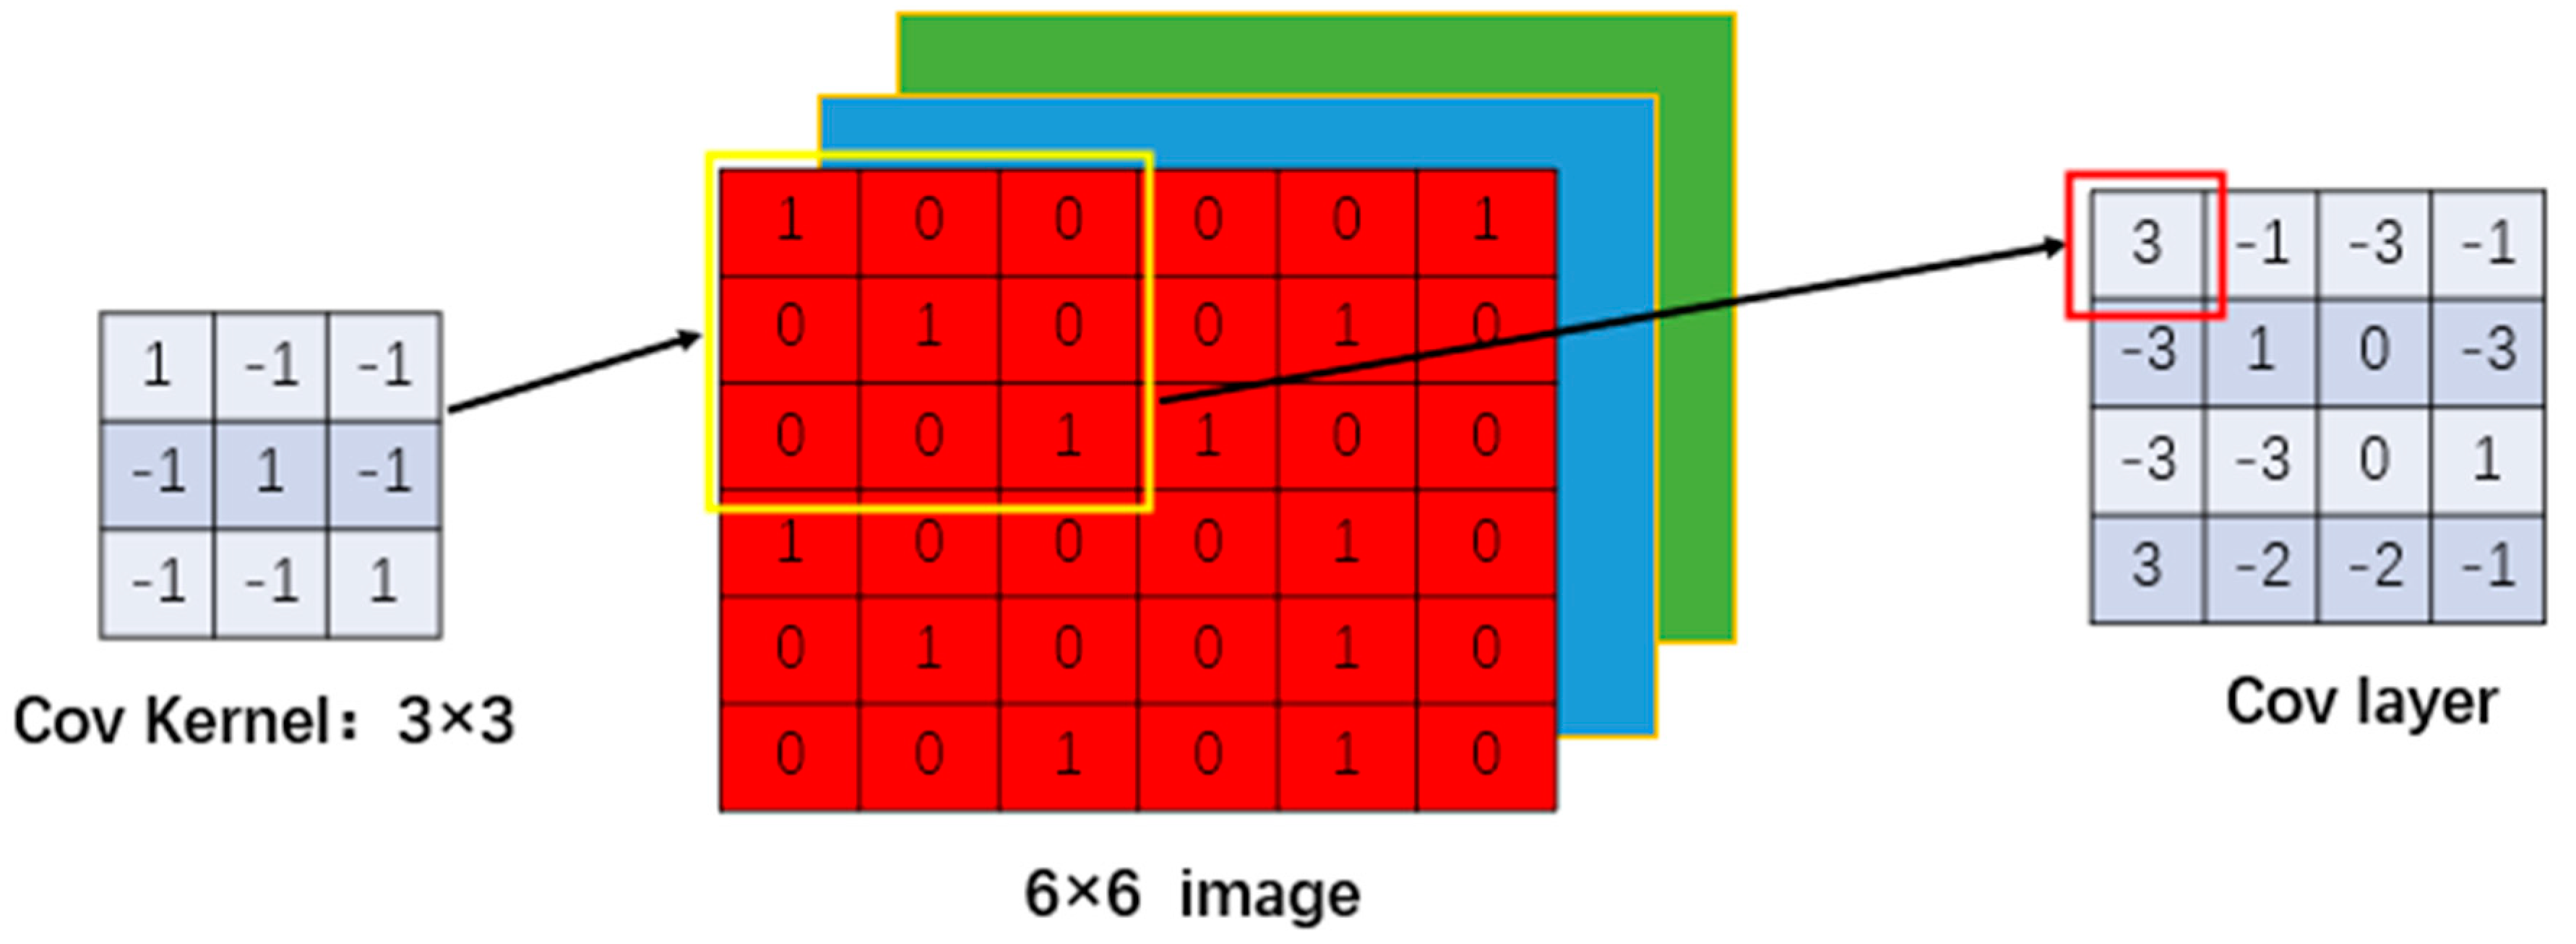
\includegraphics[width=0.60\textwidth]{Images/convlayer.jpg}
  \caption[Example of the convolution process.]{Example of the convolution process. Retrieved from \cite{review:DL}.}
  \label{fig:convlayer}
\end{figure}

Here we can also define the terms stride and padding. Stride is the number of pixels shifts over the input matrix. If the stride is 1, we move the filters by 1 pixel at a time. In Figure \ref{fig:convlayer}, we can see that the size of the output is smaller than that of the input. To keep the dimension of the output equal to the input, padding is used where zeros are symmetrically added to the input matrix \cite{guide:cnn}.

The goal of the convolution operation is to extract high-level features from the input image. The more convolutional layers or the more kernels used in each convolutional layer, the higher the number of features extracted.



\subsubsection*{Pooling Layer}

In most cases, a convolutional layer is followed by a pooling layer. The main goal of this layer is to reduce the size of the convolved feature map in order to reduce the computational costs. This is performed by sliding a two-dimensional filter over each channel of the feature map and summarising the features that lie within the region covered by the filter. There are several types of pooling operations, but the most commonly used is the max pooling which returns the maximum value from the portion of the image covered by the filter \cite{2018guide}.

\subsubsection*{Activation Functions}

One of the main parameters in a \ac{CNN} model is the activation function. This nonlinear function can be interpreted as a selection mechanism that decides whether a particular neuron should fire or not given its input. They are often placed directly after the convolutional layer to introduce non-linearity into the feature map.

There are several commonly used activation functions such as the sigmoid, \ac{Tanh}, \ac{ReLU}, \ac{Leaky ReLU} and \ac{ELU} functions. The most commonly used function in neural networks is \ac{ReLU} (Equation \ref{eq:relu}) because it is very computationally efficient, activating only a few neurons per time, it does not saturate in the positive domain, and it converges faster than the tanh and sigmoid activation functions \cite{2018activation}.

\begin{equation}
    relu(x) = \max{\{0,x\}}
    \label{eq:relu}
\end{equation}

\subsubsection*{Fully Connected Layer}

\ac{FC} Layers usually form the last few layers of the network. The input to the fully connected layer is the output of the last pooling or convolutional layer, which is flattened and then fed into the fully connected layer. The flattened vector then passes through a few more \ac{FC} layers, where the mathematical functions are normally processed. After passing through the fully connected layers, the logistic or softmax activation function is used in the last layer to determine the probability that the input belongs to a certain class (classification) \cite{guide:cnn}. Figure \ref{fig:cnn_class} shows a diagram depicting the basic \ac{CNN} architecture for image classification:

\begin{figure}[!htb]
  \centering
  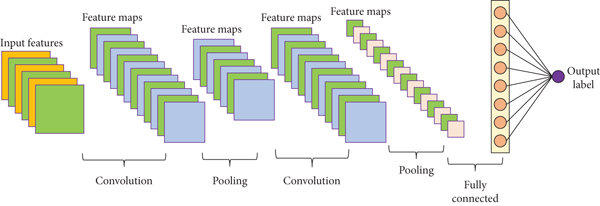
\includegraphics[width=0.75\textwidth]{Images/cnn_class.jpg}
  \caption[Basic \ac{CNN} architecture for image classification.]{Basic \ac{CNN} architecture for image classification. Retrieved from \cite{image:CNN}}
  \label{fig:cnn_class}
\end{figure}

\subsection{CNN architecture for Segmentation}

The \ac{CNN} architecture for segmentation uses encoder and decoder models. The encoders are used to downsample the spatial resolution of the input to develop a lower resolution feature mapping. The decoder then takes this feature representation as input and upsamples it to a full resolution segmentation map. The encoders can be convolutional neural networks and the decoders can be based on the deconvolutional or transposed neural networks with the purpose of creating a segmentation map \cite{enconders}. Figure \ref{fig:cnn_seg} shows the basic \ac{CNN} architecture for image segmentation.

\begin{figure}[!htb]
  \centering
  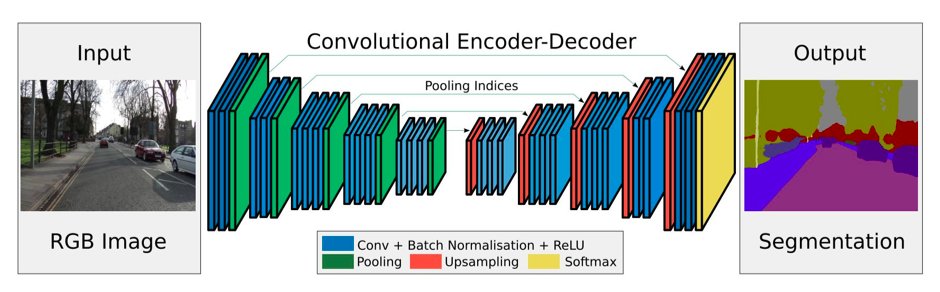
\includegraphics[width=0.75\textwidth]{Images/seg_cnn.jpg}
  \caption[Example of \ac{CNN} architecture for image segmentation.]{Example of \ac{CNN} architecture for image segmentation. Retrieved from \cite{segnet}.}
  \label{fig:cnn_seg}
\end{figure}

\subsection*{\ac{3D} \ac{CNN}}
\label{subsection:3dcnn}
In \ac{3D} \ac{CNN} architectures, the \ac{2D} convolutional and pooling layers are replaced by \ac{3D} convolutional and pooling layers. A \ac{3D} \ac{CNN} can extract more features of the volumes on the three axes X, Y, and Z. Therefore, the use of \ac{3D} information in segmentation enables the full exploitation of spatial information.

The \ac{3D} convolution kernel has one more depth than the \ac{2D} convolution kernel, the fourth dimension continues to correspond to the number of channels of the input image. Like the \ac{2D} convolution operation, a value is obtained by sliding the kernel on the height, width, and number of layers on each channel \cite{2018guide}. In figure \ref{fig:cnn_3D} the process of \ac{3D} \ac{CNN} convolution for multichannels is shown.

\begin{figure}[!htb]
  \centering
  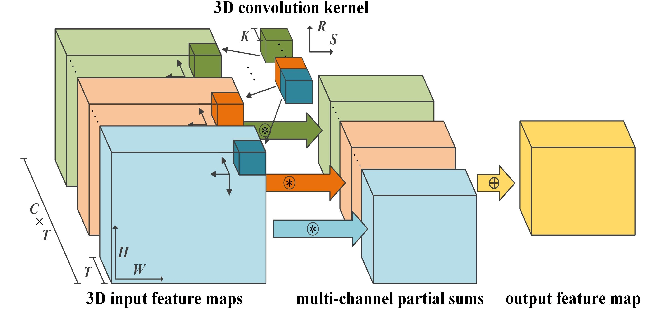
\includegraphics[width=0.65\textwidth]{Images/3dconv.jpg}
  \caption[Illustration of a \ac{3D} convolution layer]{Illustration of a \ac{3D} convolution layer. Retrieved from \cite{CNN:3D}.}
  \label{fig:cnn_3D}
\end{figure}


\subsection{CNN Training}

For training a neural network, the following steps are usually performed:

\begin{itemize}
    \item define the loss function to be minimized during training. For example, in image segmentation tasks, the most commonly used loss function is a pixel-wise cross entropy loss;
    \item select the optimizer that minimizes the loss function by defining how the parameters of the \ac{NN} are updated. The most commonly used optimizers are \ac{SGD}, \ac{SGD} with momentum, \ac{AdaGrad}, \ac{AdaDelta}, RMSProp, and \ac{ADAM}. In these optimizers, the learning rate, which controls how much the model should change in response to the estimated error each time the model weights are updated, is a hyperparameter that must be selected;
    \item split our dataset into a training, validation, and testing dataset. Use the training dataset to adjust the parameters of the model (e.g., the weights and bias in an \ac{NN}), use the validation dataset to test the model with the parameters selected during the training phase, and also use it to stop training when it stops improving (early stopping) and to adjust the hyperparameters. The test data set is used to provide an unbiased evaluation of the final fit of the model to the training data set;
    \item define the maximum number of epochs, one epoch corresponds to one run over the whole training set;
    \item define batch size, the amount of data included in each sub-epoch weight change is called the batch size. Full-batch learning uses all examples of the training set in an epoch, mini-batch learning uses only a subset of the training set, and online learning uses only one example of the training set. For example, for a training set of 100 examples, a full batch size would be 100, a mini-batch size would be 50 or 20 or 10, and an online batch size would be only 1.
    
\end{itemize}

%%%%%%%%%%%%%%%%%%%%%%%%%%%%%% U NET %%%%%%%%%%%%%%%%%%%%%%%%%%%%%%%%%%


\subsection{U-Net}

U-Net is a convolutional neural network developed by \citet{Unet:2D} for biomedical image semantic segmentation. The network is based on the \ac{FCN} \cite{fcn} and its architecture was modified and extended to work with fewer training images and to yield more precise segmentation. 

\subsubsection*{U-Net Architecture}

\begin{figure}[!htb]
  \centering
  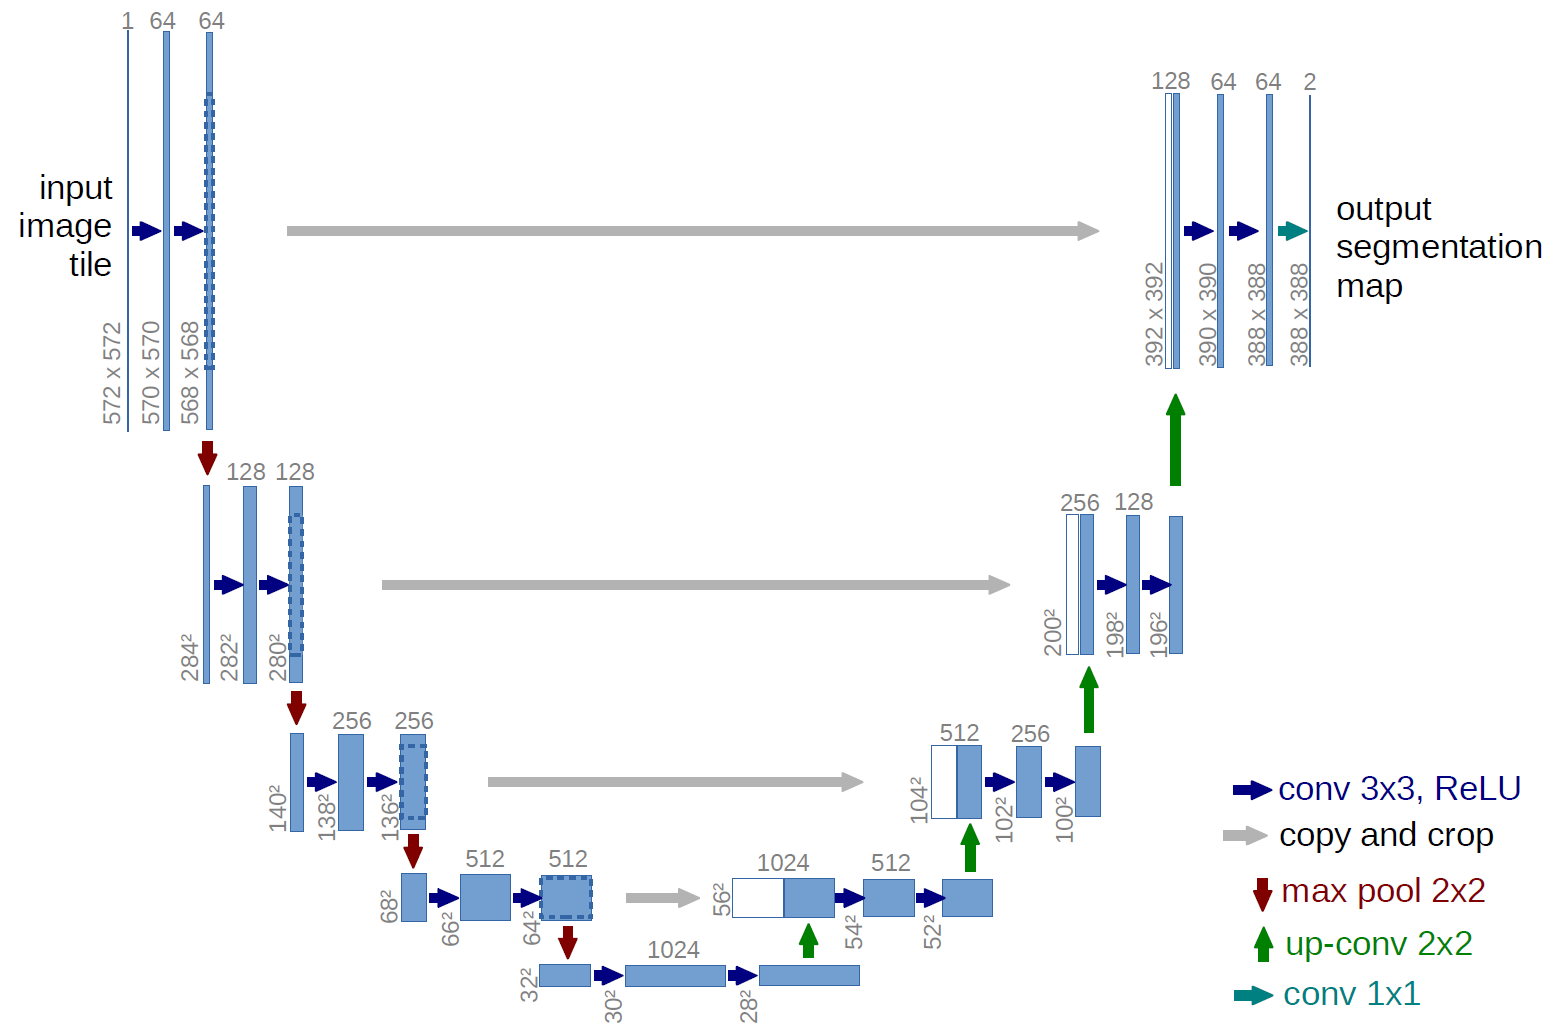
\includegraphics[width=0.85\textwidth]{Images/u-net-architecture.jpg}
  \caption[U-Net architecture.  Each blue box corresponds to a multi-channel feature map. The number of channels is denoted on top of the box. The x-y-size is provided at the lower left edge of the box. White boxes represent copied feature maps. The arrows denote the different operations.]{U-Net architecture. Each blue box corresponds to a multi-channel feature map. The number of channels is denoted on top of the box. The x-y-size is provided at the lower left edge of the box. White boxes represent copied feature maps. The arrows denote the different operations. Retrieved from \cite{Unet:2D}.}
  \label{fig:Unet:2D}
\end{figure}

The U-Net model takes its name from the fact that its architecture is in the shape of a 'U'. This architecture consists of three sections: the contraction (encoder), the bottleneck, and the expansion section (decoder). The encoder follows the typical architecture of a convolutional network. It consists of the repeated application of two unpadded 3x3 convolutions, each followed by a rectified linear unit and a 2x2 max-pooling operation with stride 2 for downsampling. At each downsampling step the number of feature channels is doubled. On this contraction path, the model captures the important features of the image and discards the unimportant ones, reducing the resolution of the image at each convolution+maxpool layer. The bottommost layer (bottleneck) mediates between the contraction layer and the expansion layer. It uses two 3x3 \ac{CNN} layers followed by 2x2 up-convolution layer.

In the expansive path, each step consists of: an upsampling of the feature map, followed by a 2x2 convolutional layer (up-convolution) that reduces the number of feature maps by half to preserve symmetry; a skip-connection and concatenation with the correspondingly cropped feature map from the contracting path, this allows valuable details learned in the encoder part to be used to construct an image in the decoder part; and two 3x3 convolutions, each followed by a \ac{ReLU}. Cropping is necessary because edge pixels are lost with each convolution. In the last layer, a 1x1 convolution is used to assign each 64-component feature vector to the desired number of classes.


\subsubsection*{Loss function}

The loss function is computed by a pixel-wise softmax over the final feature map in combination with the cross-entropy loss function. In addition, the authors introduce a weighting map into the loss function, where each pixel is assigned a weight and pixels on the boundary of segmented objects (cells in this case) have a higher weight. In this way, the network is "forced" to learn the boundary pixels.

\subsection{3D U-Net}
\label{subsection:3dunet}

\citet{Unet:3D} proposed a \ac{3D} U-Net model, as an extension of the original U-Net \cite{Unet:2D}, with the objective of making the U-Net structure have richer spatial information. The network structure is shown in figure \ref{fig:3dUnet}. 

\begin{figure}[!htb]
  \centering
  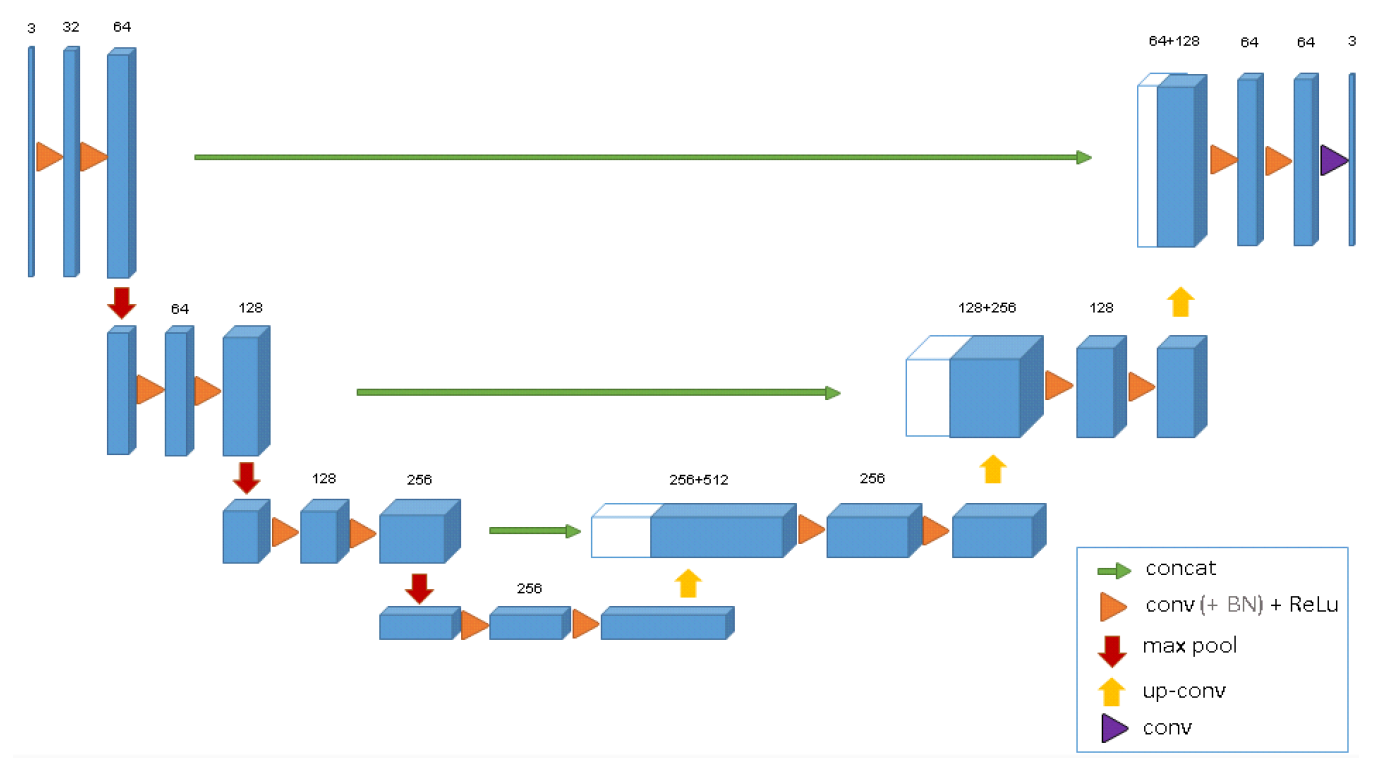
\includegraphics[width=0.85\textwidth]{Images/3dunet.jpg}
  \caption[\ac{3D} U-Net architecture.]{\ac{3D} U-Net architecture. Retrieved from \cite{Unet:3D}.}
  \label{fig:3dUnet}
\end{figure}

Similar to the \ac{2D} U-Net, the \ac{3D} U-Net architecture consists of an analysis path (left) and a synthesis path (right). The main difference is in the size of the kernels applied in the different layers (see subsection \nameref{subsection:3dcnn} for an explanation and illustration of a \ac{3D} convolutional layer). Here 3x3x3 convolutions and up-convolutions and 2x2x2 max-pooling are used, and a 1×1×1 convolution reduces the number of output channels to the number of labels. 

The authors also introduced \ac{BN} before each \ac{ReLU}. Batch normalization is a technique for training deep neural networks, where the inputs for a layer are standardized for each mini-batch. This helps to speed up the training and stabilize the learning process.

In addition, the authors continue to use softmax with weighted cross entropy as the loss function.


\section{Generative Adversarial Networks}
\label{section:GANs}
In 2014, \citet{GAN_original} introduced Generative Adversarial Networks. \ac{GANs} are an approach to generative modeling using deep learning methods, such as convolutional neural networks. Generative models capture, for a given set of data instances X and a set of labels Y, the joint probability $p(X, Y)$. In \ac{GANs}, a generative model is trained to generate realistic samples of the input data on which they have been trained.

More specifically, \ac{GANs} are algorithmic architectures inspired by game theory in which 2 neural networks, a generator and a discriminator, compete to reinforce each other. 

In a \ac{GAN}, the generator (G) is the neural network that learns the underlying distribution of the data. It receives as input a noise variable and outputs a synthetic sample. The discriminator (D) is a binary classifier that receives images as input and outputs the probability that the image is real (i.e., from the actual training set) or fake (i.e., from the generator). In this approach, the generator is trained to capture the distribution of the real data so that its generative samples are as close as possible to the real ones, or in other words, make the discriminator classify them as coming from the real dataset. The architecture of a \ac{GAN} model is shown in Figure \ref{GAN}. 

\begin{figure}[!htb]
  \centering
  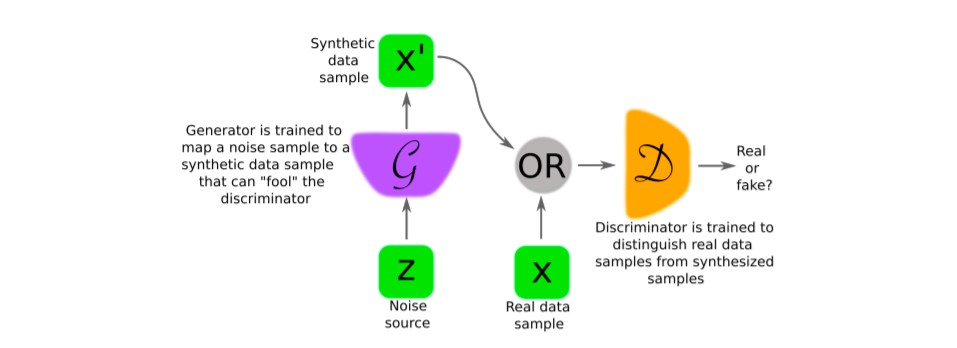
\includegraphics[width=0.90\textwidth]{Images/GAN.jpg}
  \caption[Schematic of the \ac{GAN} model. Where G and D are usually implemented as neural networks.]{Schematic of the \ac{GAN} model. Where G and D are usually implemented as neural networks. Retrieved from \cite{GAN}.}
  \label{GAN}
\end{figure}

\subsection{Training GANs}

The generator and discriminator of \ac{GANs} may have different architectures. However, since \ac{GANs} usually work with image data, they often use \ac{CNNs} as generator and discriminator models.

\subsubsection*{Loss Function}

To train a \ac{GAN}, we first need to define the loss functions of the generator and discriminator. Some notations to keep in mind are:

\begin{itemize}
    \item $p_{data}(x)$: the distribution of real data
    \item $x$: sample from $p_{data}(x)$
    \item $p(z)$: distribution of random input
    \item $z$: sample from $p(z)$
    \item $G(z)$: Generator Network
    \item $D(x)$: Discriminator Network
\end{itemize}

Since the discriminator is a binary classifier, it can be trained using the binary cross entropy loss function. As mentioned earlier, the discriminator aims to maximize the probability assigned to real and fake images. In mathematical terms, the discriminator seeks to maximize the average of the log likelihood for real images and the log value of the inverted likelihoods for fake images. Therefore, the loss function of the discriminator over a batch is given by:

\begin{equation}
    \max [\mathbb{E}_{x\sim p_{data}(x)}[\log{D(x)}]+\mathbb{E}_{z\sim p_{z}(z)}[\log{(1-D(G(z)))}]].
    \label{eq:GAN}
\end{equation}

The generator seeks to minimize the log of the inverse probability predicted by the discriminator for fake images. This has the effect of encouraging the generator to generate samples that have a low probability of being fake. This can be described as the following:

\begin{equation}
    \min [\mathbb{E}_{z\sim p_{z}(z)}[\log{(1-D(G(z)))}]].
\end{equation}

With this, we can write the final loss function as:

\begin{equation}
   \min_{G} \max_{D} [\mathbb{E}_{x\sim p_{data}(x)}[\log{D(x)}]+\mathbb{E}_{z\sim p_{z}(z)}[\log{(1-D(G(z)))}]].
\end{equation}

This means that the discriminator parameters (defined by D) maximize the loss function and the generator parameters (defined by G) minimize the loss function.

\subsubsection*{Training steps} 

The original \ac{GAN} paper provides a pseudo-code that shows how a \ac{GAN} is trained, this is shown in algorithm \ref{alg:GAN}.

\begin{algorithm}
  \scriptsize
  \caption{Minibatch stochastic gradient descent training of generative adversarial networks. Retrieved from \cite{GAN_original}.}\label{alg:GAN}
  \For{number of training iterations}{

    \For{$k$ steps}{
      \begin{itemize}
        \itemsep0em 
        \item Sample minibatch of $m$ noise samples $\left\{\boldsymbol{z}^{(1)}, \ldots, \boldsymbol{z}^{(m)}\right\}$ from noise prior $p_g(\boldsymbol{z})$.
        \item Sample minibatch of $m$ examples $\left\{\boldsymbol{x}^{(1)}, \ldots, \boldsymbol{x}^{(m)}\right\}$ from data generating distribution $p_{\text {data }}(\boldsymbol{x})$.
        \item Update the discriminator by ascending its stochastic gradient:
        $$
        \nabla_{\theta_d} \frac{1}{m} \sum_{i=1}^m\left[\log D\left(\boldsymbol{x}^{(i)}\right)+\log \left(1-D\left(G\left(\boldsymbol{z}^{(i)}\right)\right)\right)\right] .
        $$
      \end{itemize}
    }
  
    \begin{itemize}
      \itemsep0em 
      \item Sample minibatch of $m$ noise samples $\left\{\boldsymbol{z}^{(1)}, \ldots, \boldsymbol{z}^{(m)}\right\}$ from noise prior $p_g(\boldsymbol{z})$.
      \item Update the generator by descending its stochastic gradient:
      $$
      \nabla_{\theta_g} \frac{1}{m} \sum_{i=1}^m \log \left(1-D\left(G\left(z^{(i)}\right)\right)\right) .
      $$
    \end{itemize}
  }
\end{algorithm}


In the algorithm \ref{alg:GAN} it's evident that the \ac{GAN} training proceeds in alternating periods:

\begin{enumerate}
  \item The discriminator trains for $k$ steps ($k$=1 in \cite{GAN_original}), and during this period the generator is not trained;
  \item The generator is updated only after $k$ steps, and during this period the discriminator is not trained; 
  \item Repeat steps 1 and 2, for a specified number of iterations, to further train the generator and discriminator networks.
\end{enumerate}

\subsection{Supervised GAN example: Pix2Pix}
\label{subsection:pix2pix}

In recent years, several \ac{GAN} models have been proposed to perform different tasks. One of these models is Pix2Pix, which was introduced by \citet{isola2018imagetoimage} to accomplish the task of image-to-image translation.

Pix2Pix is an implementation of the \ac{cGAN}, where the generation of an image depends on another given image. The general architecture of a \ac{cGAN} model is shown in Figure \ref{fig:cGAN}.

\begin{figure}[!htb]
  \centering
  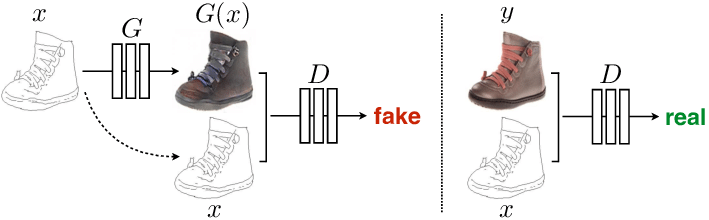
\includegraphics[width=0.70\textwidth]{Images/Training-a-conditional-GAN-to-map-edgesphoto-The-discriminator-D-learns-to-classify.jpg}
  \caption[Schematic of the \ac{cGAN} model.]{Schematic of the \ac{cGAN} model. Retrieved from \cite{isola2018imagetoimage}.}
  \label{fig:cGAN}
\end{figure}


As shown in Figure \ref{fig:cGAN}, the generator model receives a given image as input and generates a translated version of the image. The discriminator model receives an input image from the source domain and an image from the target domain and must determine whether the image from the target domain is a real or generated version of the source image. Finally, the generator model is trained to both fool the discriminator model and minimize the loss between the generated image and the expected target image. Therefore, the Pix2Pix \ac{GAN} must be trained on image datasets consisting of input images (before translation) and output or target images (after translation).


\subsubsection*{Generator and discriminator architecture}

In \cite{isola2018imagetoimage}, a U-Net model is used for the generator, and, after well trained, it takes as input an image from the source domain and outputs an image in the target domain. 

For the discriminator, the authors chose the PatchGAN discriminator. The PatchGAN, also called the Markov discriminator, classifies individual (N x N) patches in the image as real or fake, rather than classifying the entire image as real or fake. The output of the network is a single feature map of real/fake predictions that can be averaged to give a single classification score. The advantage of using a PatchGAN over a normal \ac{GAN} discriminator is that it has fewer parameters than a normal discriminator and can work with images of any size.

\subsubsection*{Loss Function}

The conditional adversarial Loss is defined as follows:

\begin{equation}
    \mathcal{L}_{cGAN}(G,D) = \mathbb{E}_{x,y} [\log{D(x,y)}] + \mathbb{E}_{x,z} [\log{(1-D(x,G(x,z)))}],
    \label{eq:1}
\end{equation}

where $x$ is the input observed image, $y$ is the real target image, $z$ is a random noise vector and $G(x,z)$ is the output generated image.

The generator model is trained using both the adversarial loss for the discriminator model and the $L_1$ or mean absolute pixel difference between the generated translation of the source image and the expected target image. The adversarial loss affects whether the generator model can output images that are plausible in the target domain, while the $L_1$ loss regularizes the generator model to output images that are plausible translations of the source image.

The L1 loss function is shown below:

\begin{equation}
    \mathcal{L}_{1}(G) = \mathbb{E}_{x,y,z} [||y-G(x,z)||_1].
    \label{eq:2}
\end{equation}

Combining these functions from \ref{eq:1} and \ref{eq:2}, results in the final objective function:

\begin{equation}
    G^* = \arg \min_{G}\max_{D} \mathcal{L}_{cGAN}(G,D) + \lambda_1  \mathcal{L}_{1}(G)
\end{equation}

where $\lambda_1$ is a hyperparameter that controls the relative importance of the L1 loss term. 

\subsection{Unsupervised GAN example: CycleGAN}
\label{subsection:CycleGAN}

As shown, the Pix2Pix model is capable of solving the image-to-image translation problem, but only if we have a paired training dataset available, i.e., a large dataset with many examples of input images X and the same image with the desired change that can be used as the expected output image Y. However, obtaining this training data is difficult in many cases. 

In 2017, \citet{cycleGAN:original} proposed a novel approach to address the unpaired image-to-image translation problem, called CycleGAN, which uses a \ac{GAN} architecture. 

As can be seen in Figure \ref{fig:cyclegan}, CycleGAN consists of two generator models, one generator (Generator 1) synthesizes images for the domain X to domain Y and the other generator (Generator 2) synthesizes images for the domain Y to domain X. Each generator has a corresponding discriminator model (Discriminator 1 and Discriminator 2). The discriminator model (1/2) takes real images from domain (Y/X) and generated images from the Generator (1/2) and predicts whether they are real or fake. 

\begin{figure}[!htb]
  \centering
  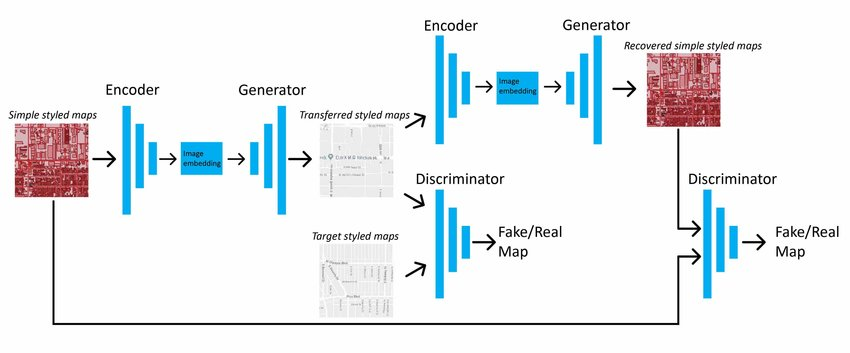
\includegraphics[width=0.90\textwidth]{Images/Data-flow-of-CycleGAN-in-this-research.jpg}
  \caption[Example of schematic of the CycleGAN model.]{Example of schematic of the CycleGAN model. Retrieved from \cite{cyclegan:image}.}
  \label{fig:cyclegan}
\end{figure}

\subsubsection*{Loss function}

The loss function used to train the generators consists of three parts: adversarial loss, cycle consistency, and identity loss. The adversarial loss  is applied to both generators. For the first \ac{GAN} (generator 1, discriminator 1), the adversarial loss is expressed as follows:

\begin{equation} \mathcal{L}_{ GAN }(G_1,D_1,X,Y)=\mathbb{E}_{y\sim p_{data}(y)}[\log{D_1(y)}]+\mathbb{E}_{x\sim p_{data}(x)}[\log{(1-D_1(G_1(x)))}]. 
\end{equation} 

For the second \ac{GAN} (generator 2, discriminator 2) is expressed as:

\begin{equation} \mathcal{L}_{ GAN }(G_2,D_2,Y,X)=\mathbb{E}_{x\sim p_{data}(x)}[\log{D_2(x)}]+\mathbb{E}_{y\sim p_{data}(y)}[\log{(1-D_2(G(y)))}]. 
\end{equation}
 
As in the original \ac{GAN} model, the generators try to minimize these losses, while the respective discriminators try to maximize them. Cycle consistency loss is a new term introduced to ensure that we preserve the original image when translating it from one domain to another and back again. Therefore, it calculates the $L_1$ loss between the original image and the generated one in two directions: $x \rightarrow G_1(x) \rightarrow G_2(G_1(x)) \approx x$ and $y \rightarrow G_2(y) \rightarrow G_1(G_2(y)) \approx y$. The cycle consistency loss is expressed as follows:

\begin{equation} 
\mathcal{L}_{cyc} = \mathbb{E}_{x\sim p_{data}(x)} [||G_{2}(G_{1}(x))-x||_1] + \mathbb{E}_{y\sim p_{data}(y)} [||G_{1}(G_{2}(y))-y||_1].
\label{eq:CCL}
\end{equation}

Finally, the identity loss is an additional optional term used mainly to preserve the color composition between input and output. It is computed by giving the generator an image of its target domain as input and computing the $L_1$ loss between input and the generated images. This loss is expressed as follows:

\begin{equation} 
\mathcal{L}_{id}(G_1,G_2) = \mathbb{E}_{y\sim p_{data}(y)} [||G_{1}(y)-y||_1] + \mathbb{E}_{x\sim p_{data}(x)} [||G_{2}(x)-x||_1].
\label{eq:identity}
\end{equation}

\section{Metrics to evaluate semantic segmentation models}

Various metrics are used to validate and test the performance of these segmentation models, the most important of which are described below.

\textbf{Pixel Accuracy} is the percentage of pixels in the image that were correctly classified. Here, a true positive/false positive (TP/FP) value represents a pixel that was correctly/incorrectly predicted as belonging to a particular class (according to the target mask), while a true negative/false negative (TN/FN) value represents a pixel that was correctly/incorrectly predicted as not belonging to a particular class.

\begin{equation}
    Accuracy = \frac{TP+TN}{TP+TN+FP+FN}
\end{equation}

\textbf{Precision} describes the \textit{purity} of positive predictions with respect to ground truth, i.e., it measures, of all the pixels predicted in a given image, how many of those pixels actually match with ground truth.

\begin{equation}
    Precision = \frac{TP}{TP+FP}
\end{equation}

\textbf{Recall} describes the \textit{completeness} of positive predictions with respect to the ground truth, i.e., of all pixels annotated in the ground truth, it measures how many of these pixels were capture as positive predictions.

\begin{equation}
    Recall = \frac{TP}{TP+FN}
\end{equation}

\textbf{\ac{IoU}} measures the similarity between two images in semantic segmentation by computing the ratio between the overlapped area and the combined area of prediction and ground truth.

\begin{equation}
    IoU = \frac{TP}{TP+FP+FN}
\end{equation}

\textbf{\ac{DC} (F1 Score)} is also used to measure the similarity between two images. It is equal to two times the overlap area between prediction and ground truth divided by the total number of pixels in both images.

\begin{equation}
    DICE = \frac{2 \ TP}{2 \ TP+FP+FN}
\end{equation}

% Escrever sobre as métricas
% https://towardsdatascience.com/metrics-to-evaluate-your-semantic-segmentation-model-6bcb99639aa2
